\section{Future Directions for Unpolarized Lepton Scattering\label{sec:directions}}

With the observations from JLab's 6~GeV era that the EMC effect may be driven by the local nuclear environment
and the apparent correspondence between the EMC effect and short range correlations, it is worth examining what
further studies with leptons scattering can be performed.
Short-range correlations offer access to understanding a more detailed picture of the high-momentum structure of nuclei as well as possible unique insight into the generation of the EMC effect.  Inclusive experiments aim to measure precision cross section ratios at $x$ above and below unity, with $x > 1$ a region forbidden to the free nucleon.  Exclusive measurements can yield a more detailed picture of the high momentum structure of nuclei, its isospin structure, and many-body correlations.


One clear avenue of exploration is to make inclusive EMC effect region measurements from additional light to medium-light
nuclei where ab-initio nuclear structure calculations are feasible and interesting nuclear cluster
structures may manifest.  One can also leverage the fact that SRCs are dominated by neutron-proton pairs to further explore
the EMC-SRC correspondence by measuring the EMC effect for a range of nuclei with
different neutron to proton ($N/P$) ratio at fixed $A$, and for a range of $A$ at fixed $N/P$ which would
expose an isovector dependence.

Inclusive $x>1$ scattering offers several unique opportunities.  Here, the lepton probes high-momentum nucleons, typically defined as ones with momenta $\ge$300~MeV/c, about a few tens of~MeV greater than the Fermi momentum for a given nucleus of $A>12$.  If the presence of these high-momentum nucleons is the result of SRCs, then the cross sections for $A>2$ will be re-scaled versions of the deuteron cross sections, signaling more SRCs and therefore more high-momentum nucleons in larger nuclei.   The observation of a plateau at $x>1$ in the $A/D$ cross-section ratios supports this picture. 

 Experimentally, the onset of the $x>1$ plateau is observed to occur at lower $x$ values as $Q^2$ increased, with the minimum $Q^2$ value taken to be about 1.4~GeV$^2$ illustrated with data from Ref.~\cite{Egiyan:2003vg}.  Cross section plateaus at $x>1$ were observed in several JLab experiments~\cite{Egiyan:2003vg, Fomin:2011ng} and is proportional to the relative number of high-momentum nucleons in $A$ with respect $D$, including the number of SRC pairs and higher order correlations.   %The pairs in a $A>2$ nucleus will experience center-of-mass motion due to the fields of the other nucleons and will redistribute some strength from the quasielastic peak to the tail of the momentum distribution, resulting in an enhancement in $A>2$ cross sections in the region of interest.  
%A convention of $a_2=\sigma_A/\sigma_D$ is used for raw cross section ratios and $R_{2N}$ for those corrected for the center-of-mass motion of the 2N pair.  

The above will be explored by JLab experiment E12-10-008~\cite{12gev_emc} in combination
with E12-06-105~\cite{12gev_xgt1}, E12-10-103~\cite{mar}, and E12-14-011~\cite{tritsrc}. E12-10-008 will measure the EMC effect for a wide range of nuclei, Fig.~\ref{fig:np_ratios},
aimed at elucidating the EMC-SRC connection, providing first measurements for a variety of light nuclei,
and exploring in-medium $N/P$ ratios via measurements of $A$ and $A\pm1$ nuclei.  E12-06-105 will make
measurements at $x>1$ in the two-nucleon correlation region for the same nuclei as well as make additional
measurements in search of possible three-nucleon correlations. Figure~\ref{fig:np_ratios} shows the $N/P$
ratio against $A$ for the nuclear targets that will be used for both experiments.%\footnote{Raphael: I suggest
%to make this a sub section of the previous section. Also a few words about EIC could be good here.}
JLab Hall A has also recently completed a campaign of data taking on the mirror nuclei $^3$H and $^3$He. 
E12-10-103 will study the ratio of the structure functions between the two nuclei and 
E12-14-011 will study their short-ranged correlations.

\begin{figure}[tbp]
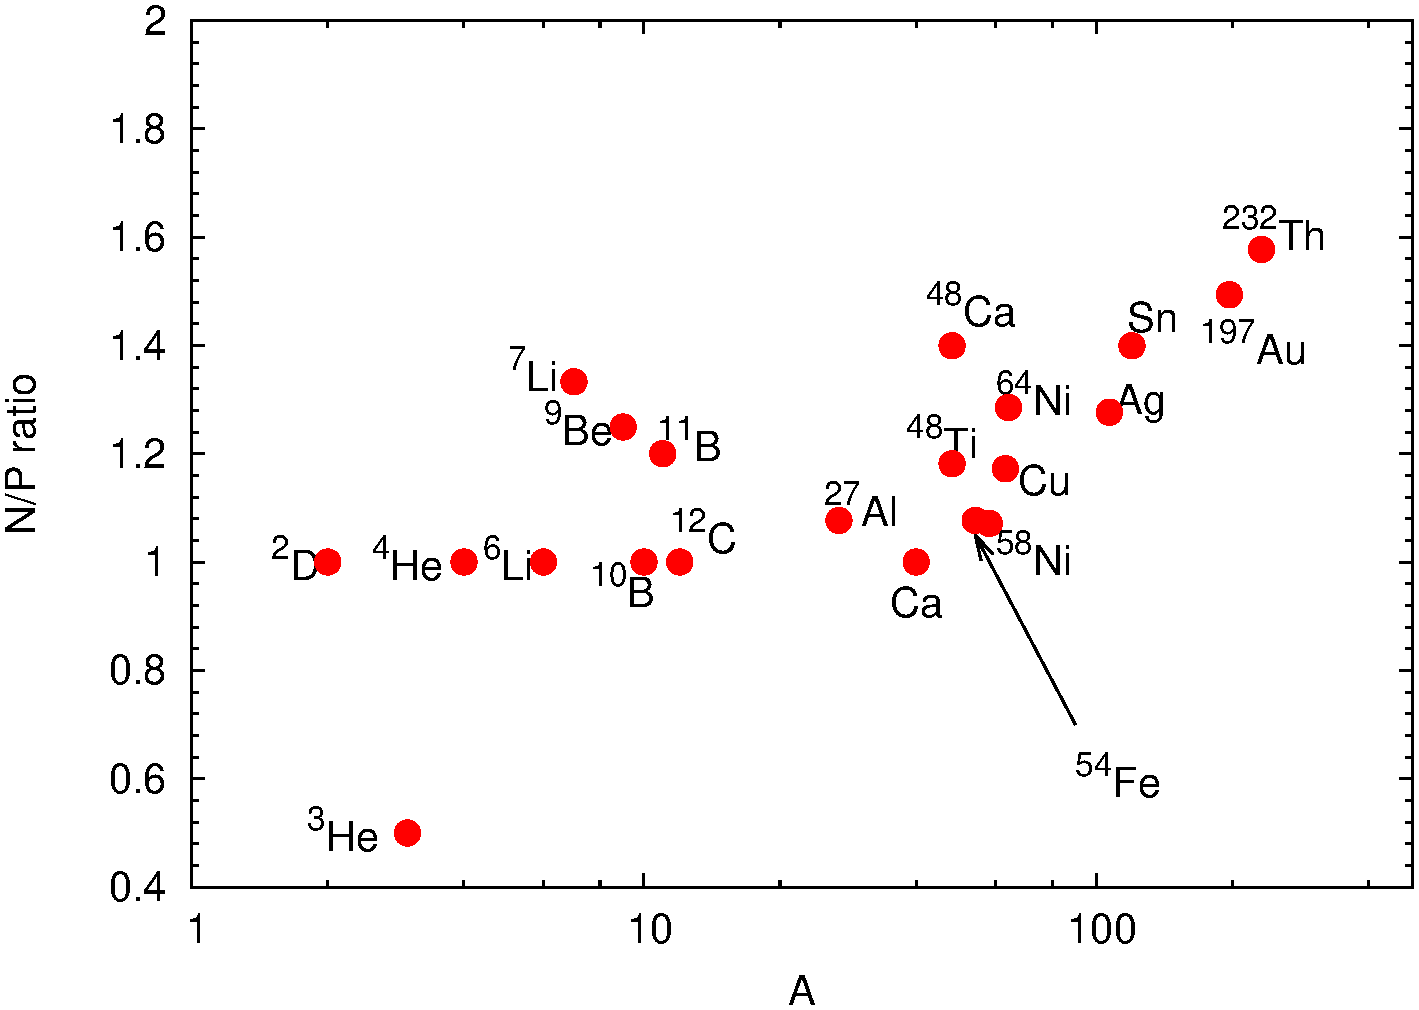
\includegraphics[width=\columnwidth,height=55mm]{plots/np_ratios_2017.pdf}
    \caption{$N/P$ ratio vs. $A$ for nuclei that will be measured by JLab experiments E12-10-008 (EMC effect), E12-06-105 ($x>1$), and E12-10-103 (MARATHON) to further elucidate the apparent link between the EMC effect and short range  correlations.}
\label{fig:np_ratios}
\end{figure}
